\section{Model Exercise 2-1a (02): Fluid driven percolation in salt}
\label{sec:mex02}
%------------------------------------------------------------------------------
\Authors{Amir Sattari, Matthias Nest, Keita Yoshioka et al.}
%------------------------------------------------------------------------------
Model Exercise 2 (ME 2) investigates the fluid driven percolation (hydraulic fracking) in salt and clay stone samples under anisotropic confining stresses. The pressurized oil is injected through the pre-drilled cavity until the sudden pressure drop or increase in flow rate is observed. The main goal of this test is to determine the stress dependent fracking path and the required fracking pressure which is slightly above the minimum principle stress applied to the system. For the simulation of the fluid driven percolation, the continuum and discreet numerical methods are considered.
%------------------------------------------------------------------------------
\subsection{Experimental set-up}
%------------------------------------------------------------------------------
The experimental tests on saltstone samples are conducted at TU Freiberg \cite{Kamlot2009}. The cubic samples with a side length dimension of 100 §mm§ are prepared and placed in the true tri-axial apparatus \ref{fig:Amir_ME2_Saltstone_Setup}. The cubic samples are prepared with a drilled cavity length and diameter of 40 and 16 $mm$, respectively. The pressurized fluid is injected through a tubing from upper boundary and the fracking and change of flow rate is tracked. The applied two anisotropic stress configurations and the fracking paths are shown in \ref{fig:Amir_ME2_stress_state_a} and \ref{fig:Amir_ME2_stress_state_b}. The figure \ref{fig:Amir_ME2_Pressure_Time_a} and \ref{fig:Amir_ME2_Pressure_Time_b} depict the change of pressure inside of the borehole with time under the constant flow rate sequels.

\begin{figure}[!ht]
\centering
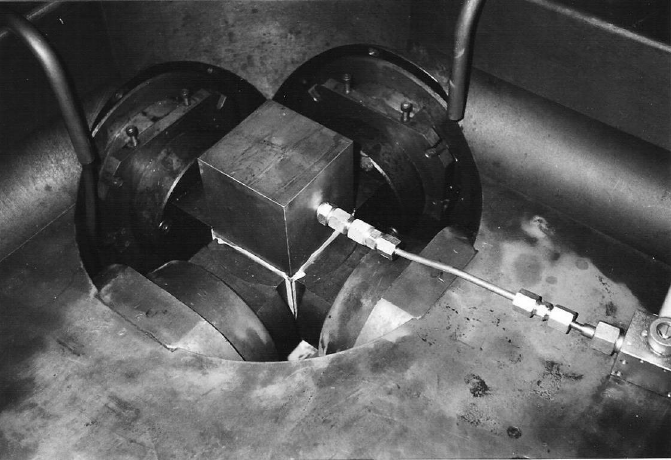
\includegraphics[width=0.5\textwidth]{figures/Amir_ME2_Saltstone_Setup.png}
\caption{ME2 setup configuration of salt stone placed inside the true tri-axial apparatus \cite{Kamlot2009}}
\label{fig:Amir_ME2_Saltstone_Setup}
\end{figure}

\begin{figure}[!ht]
\begin{subfigure}[c]{0.48\textwidth}
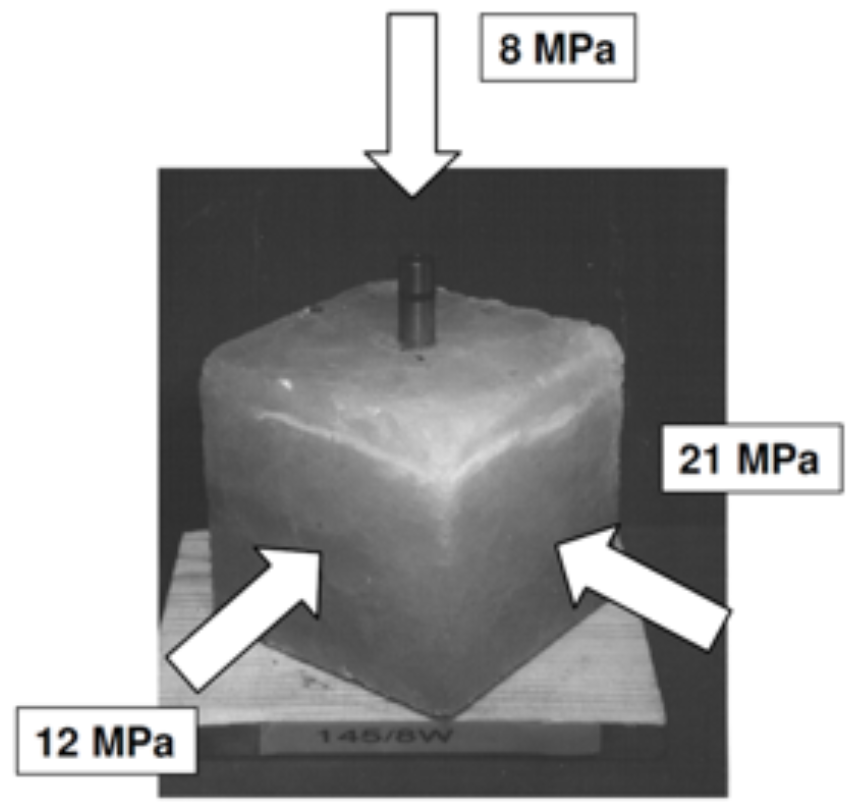
\includegraphics[width=1\textwidth]{figures/Amir_ME2_stress_state_1.png}
\subcaption{}
\label{fig:Amir_ME2_stress_state_a}
\end{subfigure}
\hfill
\begin{subfigure}[c]{0.48\textwidth}
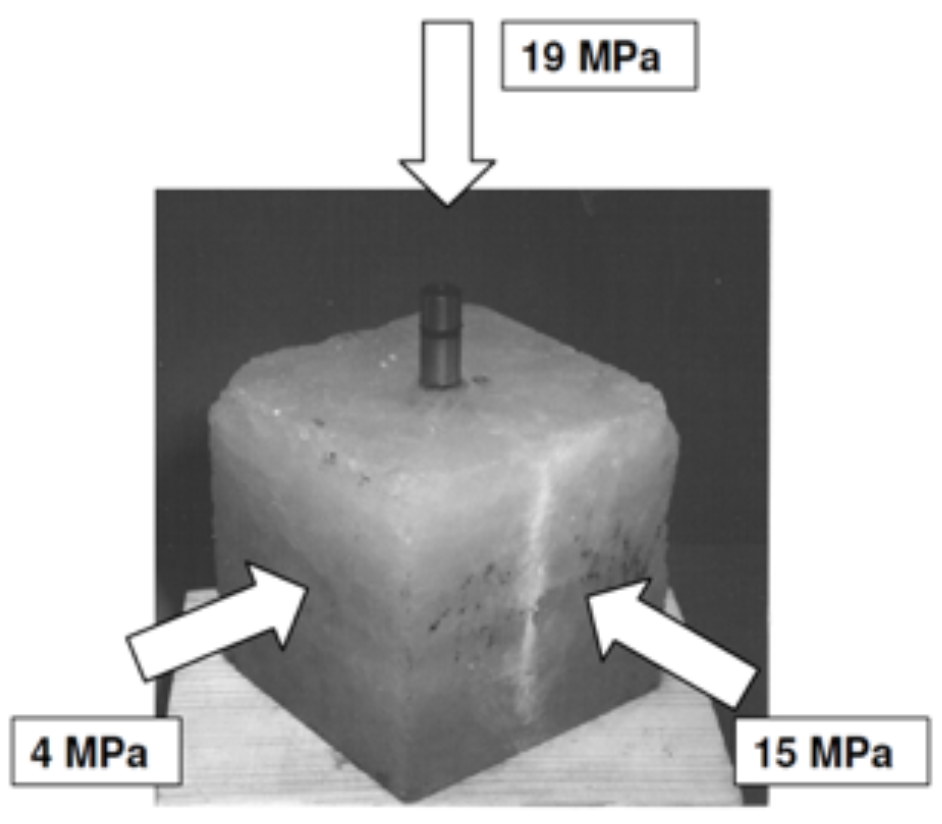
\includegraphics[width=1\textwidth]{figures/Amir_ME2_stress_state_2.png}
\subcaption{}
\label{fig:Amir_ME2_stress_state_b}
\end{subfigure}
\caption{The confining (a) 1st stress, and (b) 2nd stress configuration setup in saltstone \cite{Kamlot2009}}
\end{figure}

\begin{figure}[!ht]
\begin{subfigure}[c]{0.48\textwidth}
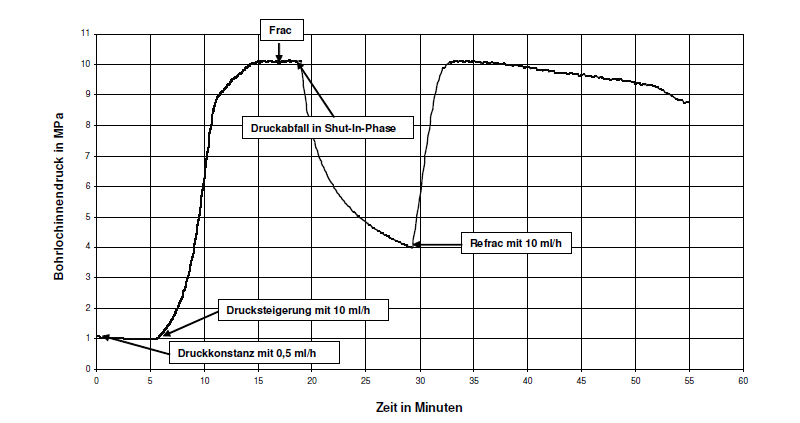
\includegraphics[width=1\textwidth]{figures/Amir_ME2_Pressure_Time_1.png}
\subcaption{}
\label{fig:Amir_ME2_Pressure_Time_a}
\end{subfigure}
\hfill
\begin{subfigure}[c]{0.48\textwidth}
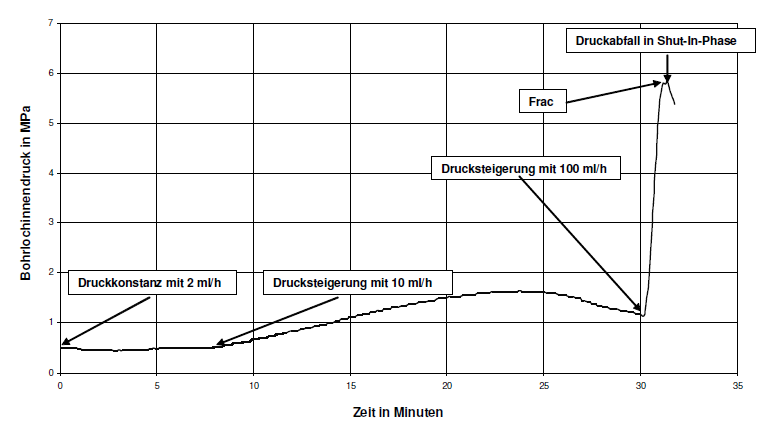
\includegraphics[width=1\textwidth]{figures/Amir_ME2_Pressure_Time_2.png}
\subcaption{}
\label{fig:Amir_ME2_Pressure_Time_b}
\end{subfigure}
\caption{The borehole pressure evolution under constant flow rate sequels for (a) 1st stress, and (b) 2nd stress configurations \cite{Kamlot2009}}
\end{figure}
%------------------------------------------------------------------------------
\subsection{Model approaches}
%------------------------------------------------------------------------------
Different numerical methods (DEM, LEM, PFM) are implemented to investigate the applicability of each model to simulate the fracking path, fracking pressure and flow rate changes in the saltstone samples. Below, the description of each model and the discussion of the results are provided. The stress dependent fracking path due to anisotropic stress configurations are captured by both continuum and discrete models. 
%------------------------------------------------------------------------------
\subsubsection*{Discrete-Element-Model (DEM)}
Figure \ref{fig:ME2_DEM_model_setup} shows the elements and interfaces/grain boundaries used for DEM simulation of the modeling exercise 2. For both of the stress states, the identical elements and interfaces were used. Simulation results from the first stress configuration are shown in \ref{fig:ME2_DEM_stress1_result}.

\begin{figure}[!ht]
\centering
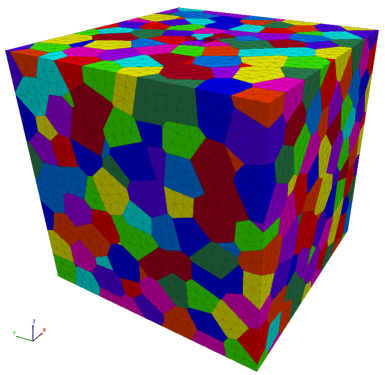
\includegraphics[width=0.45\textwidth]{figures/ME2_DEM_model.pdf}
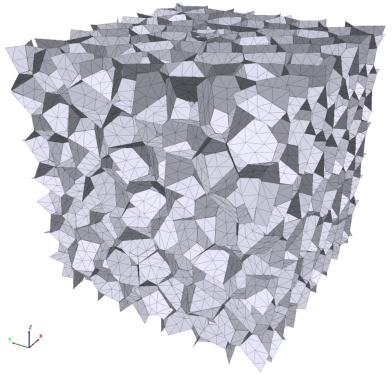
\includegraphics[width=0.45\textwidth]{figures/ME2_DEM_grain.pdf}
\caption{ME2 DEM model set-up.}
\label{fig:ME2_DEM_model_setup}
\end{figure}

\begin{figure}[!ht]
\centering
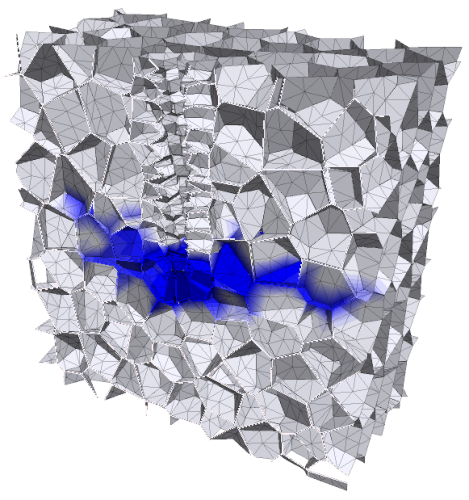
\includegraphics[width=0.45\textwidth]{figures/ME2_DEM_stress1_vertical.pdf}
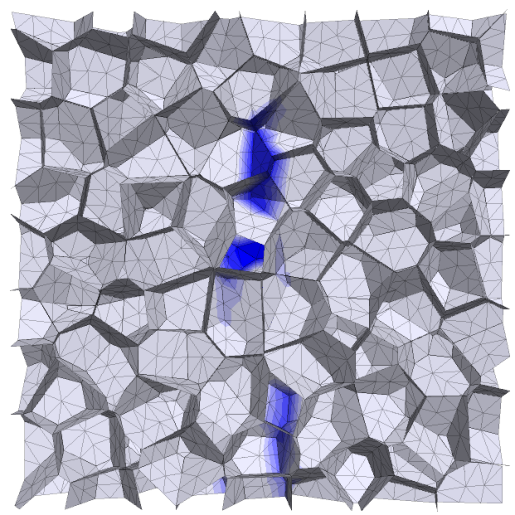
\includegraphics[width=0.45\textwidth]{figures/ME2_DEM_stress2_side.pdf}
\caption{ME2 DEM model results for the stress configuration 2.}
\label{fig:ME2_DEM_stress1_result}
\end{figure}

\begin{figure}[!ht]
\centering
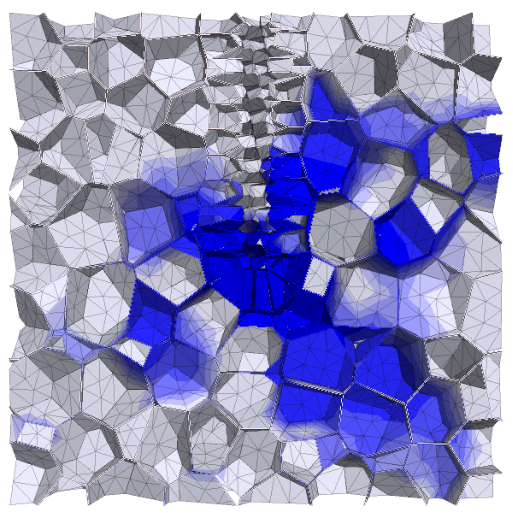
\includegraphics[width=0.45\textwidth]{figures/ME2_DEM_stress2_vertical.pdf}
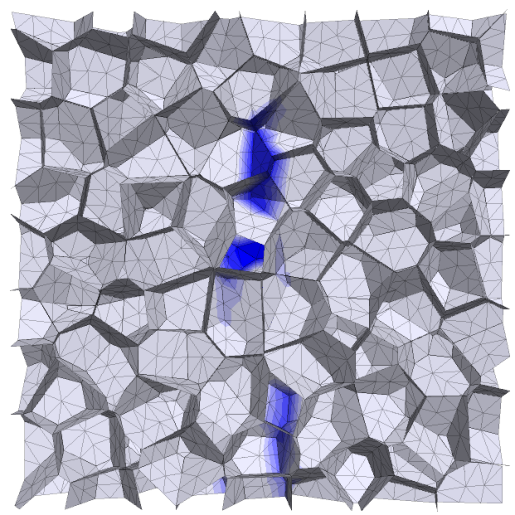
\includegraphics[width=0.45\textwidth]{figures/ME2_DEM_stress2_side.pdf}
\caption{ME2 DEM model results for the stress configuration 2.}
\label{fig:ME2_DEM_stress2_result}
\end{figure}

\subsubsection*{Lattice-Element-Model (LEM)}

The dual lattice model, described in the section \ref{Section:HMLattice}, is implemented to simulate the fluid driven percolation in the saltstone samples. The applied hydraulic pressures are transformed into the mechanical model using the weak coupling scheme and subsequently the elements failure and change of hydraulic aperture are determined and transformed back to the hydro model. The considered mass conservation methodology results in the prediction of flow rate and change of reservoirs pressure as well as the flow and fracking paths which are then compared to the experimental data. The total number of mechanical and conduct lattice elements are 10000 and 80000, respectively (\ref{fig:Amir_ME2_LEM_a_model}).  The experimental setup shown in \ref{fig:Amir_ME2_stress_state_a} is simulated using  the dual LEM and the developed fractures and flow path are shown in \ref{fig:Amir_ME2_LEM_a_model_Fracture} and \ref{fig:Amir_ME2_LEM_a_model_Flow}. Similarly, the fracture surfaces and flow paths under the second stress configuration \ref{fig:Amir_ME2_stress_state_b} are illustrated in \ref{fig:Amir_ME2_LEM_b_model_Fracture} and \ref{fig:Amir_ME2_LEM_b_model_Flow}, respectively. 

\begin{figure}[!ht]
\centering
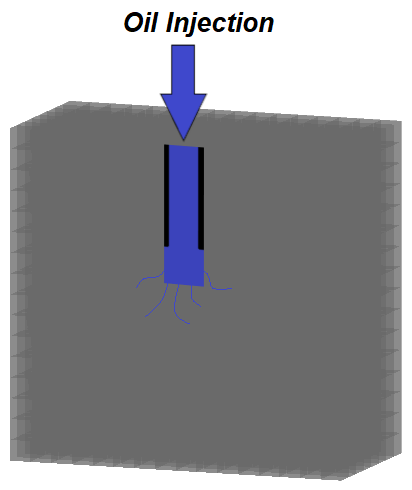
\includegraphics[width=0.5\textwidth]{figures/Amir_ME2_LEM_a_model.png}
\caption{The initial stress configuration in dual LEM.}
\label{fig:Amir_ME2_LEM_a_model}
\end{figure}

\begin{figure}[!ht]
\begin{subfigure}[c]{0.48\textwidth}
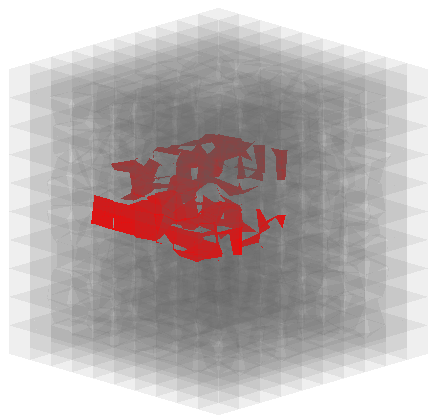
\includegraphics[width=1\textwidth]{figures/Amir_ME2_LEM_a_model_Fracture.png}
\subcaption{}
\label{fig:Amir_ME2_LEM_a_model_Fracture}
\end{subfigure}
\hfill
\begin{subfigure}[c]{0.48\textwidth}
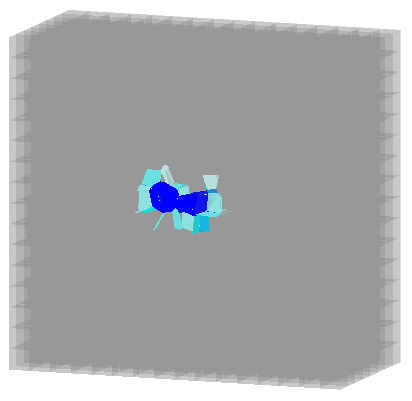
\includegraphics[width=1\textwidth]{figures/Amir_ME2_LEM_a_model_Flow.png}
\subcaption{}
\label{fig:Amir_ME2_LEM_a_model_Flow}
\end{subfigure}
\caption{ The simulation of fluid driven percolation shown in \ref{fig:Amir_ME2_stress_state_a}: The cross-section of the (a) fracking surfaces (red), and (b) flow transport surfaces (blue)}
\end{figure}

\begin{figure}[!ht]
\begin{subfigure}[c]{0.48\textwidth}
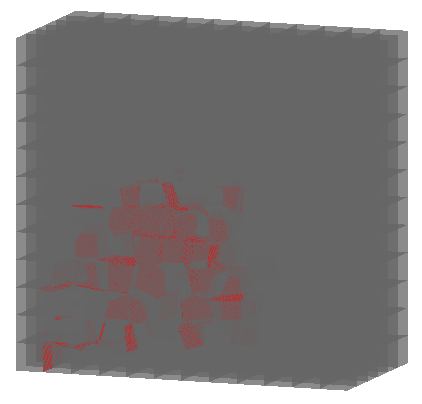
\includegraphics[width=1\textwidth]{figures/Amir_ME2_LEM_b_model_Fracture.png}
\subcaption{}
\label{fig:Amir_ME2_LEM_b_model_Fracture}
\end{subfigure}
\hfill
\begin{subfigure}[c]{0.48\textwidth}
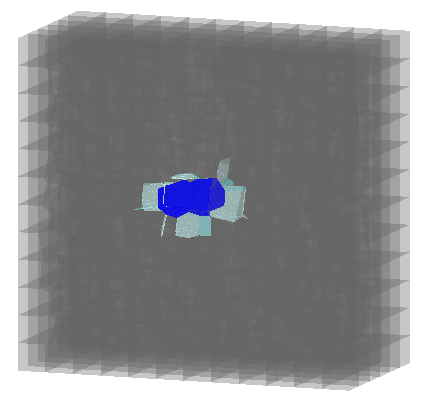
\includegraphics[width=1\textwidth]{figures/Amir_ME2_LEM_b_model_Flow.png}
\subcaption{}
\label{fig:Amir_ME2_LEM_b_model_Flow}
\end{subfigure}
\caption{ The simulation of fluid driven percolation shown in \ref{fig:Amir_ME2_stress_state_b}: The cross-section of the (a) fracking surfaces (red), and (b) flow transport surfaces (blue)}
\end{figure}
%------------------------------------------------------------------------------
\subsubsection*{Finite-Element-Model: Variational-Phase-Field (VPF)}
%------------------------------------------------------------------------------
\todo[inline]{[UFZ](KY): Please add results}
%------------------------------------------------------------------------------
\subsection{Results and discussion}
%------------------------------------------------------------------------------
\todo[inline]{[CAU]: Please add discussion}
%------------------------------------------------------------------------------

